\documentclass[a4paper,12pt]{article}
\usepackage[left=2cm,right=2cm,top=2cm,bottom=2cm]{geometry} % Do ustawień marginesów
\usepackage{multicol} % Dla podziału na kolumny
\usepackage{ragged2e} % Dla justowania tekstu
\usepackage{graphicx} % Required for inserting images
\usepackage{float}
\usepackage{caption}
\usepackage{amsmath} % Math formulas
\usepackage{amssymb} % Symbols
\usepackage[svgnames]{xcolor}
\usepackage[colorlinks=true, urlcolor=blue, linkcolor=black, citecolor=orange]{hyperref} % Hyperlinks
\usepackage{polski} % Polish language
\usepackage[utf8]{inputenc} % Text encoding
\usepackage{enumitem} % Pakiet do elastycznego sterowania listami
\usepackage{indentfirst}
\usepackage{array}

\begin{document}

% Górna część strony
\noindent
\begin{minipage}{0.5\textwidth}
    \raggedright
    \textbf{Piotr Durniat} \\
    I rok, Fizyka \\
    Wtorek, 8:00-10:15 \\
    \vspace{0.5cm}
    \vspace{0.5cm}
\end{minipage}%
\begin{minipage}{0.5\textwidth}
    \raggedleft
    Data wykonania pomiarów: \\
    01.04.2025 \\
    \vspace{0.5cm} % Dodatkowa linia przerwy
    Prowadząca: \\
    dr Iwona Mróz
\end{minipage}

% Tytuł ćwiczenia
\vspace{2cm} % Odstęp
\begin{center}
    \LARGE \textbf{Ćwiczenie nr 15} \\[0.5cm]
    \Large \textbf{Drgania masy zawieszonej na sprężynie}
\end{center}

% Reszta treści
\vspace{1cm} % Kolejny odstęp
\noindent

\tableofcontents
\newpage

% ---------- WSTĘP TEORETYCZNY ----------
\section{Wstęp teoretyczny}

% ---------- OPIS DOŚWIADCZENIA ----------
\section{Opis doświadczenia}

% ---------- OPRACOWANIE WYNIKÓW POMIARÓW ----------
\section{Opracowanie wyników pomiarów}

% ---------- TABELE ----------
\subsection{Tabele pomiarowe}




\begin{table}[H]
    \centering
    \begin{tabular}{|c|c|c|}
        \hline
        Nr & $A$ [cm] & $t(20 \text{ drgań})$ [s] \\
        \hline
        1  & 1 & 31,50 \\
        2  & 2 & 31,31 \\
        3  & 3 & 31,41 \\
        4  & 4 & 31,50 \\
        5  & 5 & 31,31 \\
        6  & 6 & 31,43 \\
        7  & 7 & 31,44 \\
        8  & 8 & 31,28 \\
        9  & 9 & 31,34 \\
        10 & 10 & 31,50 \\
        \hline
    \end{tabular}
    \caption{Zależność okresu drgań od amplitudy}
\end{table}

\begin{table}[H]
    \centering
    \begin{tabular}{|c|c|}
        \hline
        Nr & $t(20 \text{ drgań})$ [s] \\
        \hline
        1 & 31,44 \\
        2 & 31,16 \\
        3 & 31,28 \\
        4 & 31,34 \\
        5 & 31,66 \\
        \hline
    \end{tabular}
    \caption{Pomiar okresu dla $A = 5 \text{ cm}$}
    \label{tab:okres_5cm}
\end{table}

\begin{table}[H]
    \centering
    \begin{tabular}{|c|c|c|}
        \hline
        Nr & $m$ [g] & $x$ [cm] \\
        \hline
        1  & 10  & 21,0 \\
        2  & 20  & 28,2 \\
        3  & 30  & 35,4 \\
        4  & 40  & 42,6 \\
        5  & 50  & 50,0 \\
        6  & 60  & 57,1 \\
        \hline
        7  & 60  & 57,1 \\
        8  & 50  & 50,0 \\
        9  & 40  & 42,8 \\
        10 & 30  & 35,5 \\
        11 & 20  & 28,2 \\
        12 & 10  & 21,0 \\
        \hline
    \end{tabular}
    \caption{Zależność położenia szalki od masy}
\end{table}

\begin{table}[H]
    \centering
    \begin{tabular}{|c|c|c|}
        \hline
        $m$ [g] & $t(20 \text{ drgań})\,[\text{s}]$ & $t(10 \text{ drgań})\,[\text{s}]$ \\
        \hline
        10 & 25,41 & 12,81 \\
        20 & 26,13 & 13,94 \\
        30 & 29,53 & 14,81 \\
        40 & 31,47 & 15,59 \\
        50 & 33,06 & 16,60 \\
        60 & 34,72 & 17,84 \\
        $m_x$ & 33,22 & 14,91 \\
        \hline
    \end{tabular}
    \caption{Zależność okresu drgań od masy}
\end{table}



% ---------- OBLICZENIA ----------
\subsection{2.  Zakres stosowalności prawa Hooke'a}


Dla szalki bez obciążenia położenie wynosi $x_0 = 13.6$ cm.
Na podstawie wyników obliczono wydłużenie $\Delta x_i$ jako różnicę między położeniem przy obciążeniu a położeniem początkowym:

\begin{equation}
    \label{eq:wydluzenie}
    \Delta x_i = x_i - x_0
\end{equation}

Następnie obliczono średnie wartości wydłużeń sprężyny \(x_i\) pod wpływem określonych obciążeń zgodnie ze wzorem:

\begin{equation*}
    \overline{\Delta x_i} = \frac{\Delta x_{i1} + \Delta x_{i2}}{2}
\end{equation*}

gdzie:
\begin{itemize}
    \setlength{\itemsep}{0em}
    \item \(\Delta x_{i1}\) -- wydłużenie szalki z masą \(m_i\) przy obciążeniu rosnącym,
    \item \(\Delta x_{i2}\) -- wydłużenie przy obciążeniu malejącym.
\end{itemize}

Wyniki obliczeń wydłużeń przedstawiono w tabeli \ref{tab:delta_x}.

\begin{table}[H]
    \centering
    \begin{tabular}{|c|c|c|}
        \hline
        $m$ [kg] & $\Delta x_1$ [m] & $\Delta x_2$ [m] \\
        \hline
        0,010 & 0,074 & 0,074 \\
        0,020 & 0,146 & 0,146 \\
        0,030 & 0,218 & 0,219 \\
        0,040 & 0,290 & 0,292 \\
        0,050 & 0,364 & 0,364 \\
        0,060 & 0,435 & 0,435 \\
        \hline
    \end{tabular}
    \caption{Wartości wydłużeń sprężyny}
    \label{tab:delta_x}
\end{table}

Ciężar $F$ został obliczony ze wzoru:

\begin{equation*}
    F = mg
\end{equation*}

gdzie:
\begin{itemize}
    \setlength{\itemsep}{0em}
    \item $m$ -- masa odważnika [kg],
    \item $g$ -- przyspieszenie ziemskie [m/s$^2$].
\end{itemize}

W obliczeniach przyjęto wartość przyspieszenia ziemskiego $g = 9,81$ m/s$^2$.
Wyniki obliczeń przedstawiono w tabeli \ref{tab:wydluzenia}.
Wykres zależności wydłużenia sprężyny od ciężaru przedstawiono na rysunku \ref{fig:zaleznosci}.

\begin{table}[H]
    \centering
    \begin{tabular}{|c|c|c|}
        \hline
        $m$ [kg] & $F$ [N] & $\overline{\Delta x}$ [m] \\
        \hline
        0,010 & 0,0981 & 0,074 \\
        0,020 & 0,1962 & 0,146 \\
        0,030 & 0,2943 & 0,2185 \\
        0,040 & 0,3924 & 0,291 \\
        0,050 & 0,4905 & 0,364 \\
        0,060 & 0,5886 & 0,435 \\
        \hline
    \end{tabular}
    \caption{Średnie wartości wydłużeń sprężyny}
    \label{tab:wydluzenia}
\end{table}

\subsubsection{Współczynnik sprężystości}

W celu wyznaczenia współczynnika sprężystości sprężyny zastosowano regresję liniową dla zależności wydłużenia $\Delta x$ od siły $F$ wykorzystując język Python i bibliotekę NumPy. Na podstawie równania regresji:

\begin{equation*}
    \Delta x = kF + b
\end{equation*}

gdzie:
\begin{itemize}
    \setlength{\itemsep}{0em}
    \item $k$ -- współczynnik sprężystości [m/N],
    \item $b$ -- wyraz wolny [m].
\end{itemize}

otrzymano następujące wartości:
\begin{itemize}
    \setlength{\itemsep}{0em}
    \item $k = 0,7373$ m/N,
    \item $b = 0,00160$ m.
\end{itemize}


% ---------- NIEPEWNOŚCI ----------
\section{Ocena niepewności pomiaru}

\subsection{Niepewność czasu}

Niepewność typu B czasu obliczono ze wzoru:

\begin{equation*}
    u_B(t) = \frac{\Delta_d(t)}{\sqrt{3}}
\end{equation*}

Gdzie $\Delta_d(t) = 0.2$ to błąd eksperymentatora, stąd:

\begin{equation*}
    u_B(t) = \frac{0.2}{\sqrt{3}} \approx 0.12 \text{ s}
\end{equation*}

Niepewność typu A czasu wyznaczono na podstawie pięciu powtórzonych pomiarów dla amplitudy 5 cm (tabela \ref{tab:okres_5cm}), wykorzystując wzór \ref{eq:niepewnosc_A}.

\begin{equation} \label{eq:niepewnosc_A}
    u_A(t) = \sqrt{\frac{1}{n-1} \sum_{i=1}^{n} (t_i - \bar{t})^2}
\end{equation}

Podstawiając wartości do wzoru \ref{eq:niepewnosc_A} otrzymano:

\begin{equation*}
    u_A(t) = 0.19 \text{ s}
\end{equation*}

Niepewność złożoną czasu obliczono ze wzoru:

\begin{equation*}
    u_c(t) = \sqrt{u_A(t)^2 + u_B(t)^2}
\end{equation*}

Podstawiając wartości do wzoru otrzymano:

\begin{equation*}
    u_c(t) = \sqrt{0.19^2 + 0.12^2} \approx 0.22 \text{ s}
\end{equation*}





\subsection{Niepewność okresu}

Okres obliczono ze wzoru:

\begin{equation*}
    T = \frac{t}{N}
\end{equation*}

Gdzie $N$ to liczba drgań, stąd:

\begin{equation*}
    u_c(T) = \frac{u_c(t)}{N}
\end{equation*}

podstawiając wartość niepewności czasu otrzymano:

\begin{equation*}
    u_c(T) = \frac{0.22}{20} \approx 0.011 \text{ s}
\end{equation*}


\subsection{Niepewność położenia}

Niepewność maksymalna miarki wynosi $\Delta_d = 0.001$ m. Niepewność wydłużenia obliczono ze wzoru:

\begin{equation*}
    u_B(x) = \frac{\Delta_d x}{\sqrt{3}}
\end{equation*}

Po podstawieniu wartości otrzymano:

\begin{equation*}
    u_B(x) = \frac{0.001}{3} = 0.00058 \text{ m}
\end{equation*}

\subsection{Niepewność wydłużenia}

Niepewność wydłużenia obliczono z prawa przenoszenia niepewności dla wzoru \ref{eq:wydluzenie}:

\begin{align*}
    u_c(\Delta x) & = \sqrt{\left(\frac{\partial \Delta x}{\partial x}\right)^2 u^2(x) + \left(\frac{\partial \Delta x}{\partial x_0}\right)^2 u^2(x_0)} \\
                  & = \sqrt{(1)^2 u^2(x) + (-1)^2 u^2(x_0)}                                                                                              \\
                  & = \sqrt{2} u_B(x)
\end{align*}

Stąd niepewność pojedynczego pomiaru wydłużenia:

\begin{equation*}
    u_c(\Delta x) = \sqrt{2} \cdot 0.00058 \approx 0.00082 \text{ m}
\end{equation*}

\subsection{Niepewność średniego wydłużenia}

\subsection*{Niepewność złożona średniego wydłużenia}

Dla średniego wydłużenia:
\begin{equation*}
    \overline{\Delta x_i} = \frac{\Delta x_{i1} + \Delta x_{i2}}{2}
\end{equation*}

niepewność złożoną możemy wyznaczyć korzystając z prawa propagacji niepewności:

\begin{align*}
    u_c(\overline{\Delta x_i}) & = \sqrt{\left(\frac{\partial \overline{\Delta x_i}}{\partial \Delta x_{i1}}\right)^2 u^2(\Delta x_{i1}) + \left(\frac{\partial \overline{\Delta x_i}}{\partial \Delta x_{i2}}\right)^2 u^2(\Delta x_{i2})} \\
                               & = \sqrt{\left(\frac{1}{2}\right)^2 u^2(\Delta x) + \left(\frac{1}{2}\right)^2 u^2(\Delta x)}                                                                                                               \\
                               & = \sqrt{\frac{2}{4} u^2(\Delta x)} = \frac{u(\Delta x)}{\sqrt{2}}
\end{align*}

Podstawiając wartość niepewności pojedynczego pomiaru wydłużenia otrzymano:

\begin{equation*}
    u_c(\overline{\Delta x_i}) = \frac{0.00082}{\sqrt{2}} \approx 0.00058 \text{ m}
\end{equation*}


\subsection{Współczynnik sprężystości}

Niepewności współczynników regresji liniowej obliczono na podstawie następujących wzorów:

\[
    s_y = \sqrt{\frac{\sum_{i=1}^{n} (y_i - \hat{y}_i)^2}{n-2}}
\]

\[
    u(k) = s_y \sqrt{\frac{n}{n \sum x_i^2 - \left( \sum x_i \right)^2}}
\]

\[
    u(b) = s_y \sqrt{\frac{\sum x_i^2}{n \sum x_i^2 - \left( \sum x_i \right)^2}}
\]

gdzie:

\begin{itemize}
    \setlength{\itemsep}{0em}
    \item $s_y$ -- odchylenie standardowe reszt,
    \item $u(k)$ -- niepewność standardowa współczynnika kierunkowego prostej regresji,
    \item $u(b)$ -- niepewność standardowa wyrazu wolnego prostej regresji,
    \item $n$ -- liczba punktów pomiarowych,
    \item $x_i$ -- wartości zmiennej niezależnej (siła $F$),
    \item $y_i$ -- wartości zmierzone (wydłużenie $\Delta x$),
    \item $\hat{y}_i$ -- wartości przewidywane przez model regresji,
\end{itemize}

Obliczone wartości niepewności dla współczynników prostej regresji wynoszą:

\begin{itemize}
    \setlength{\itemsep}{0em}
    \item $u(k) = 0.0012\,\frac{\text{m}}{\text{N}}$
    \item $u(b) = 0.00046\,\text{m}$
\end{itemize}


% ---------- WNIOSKI ----------
\section{Wnioski}

% ---------- WYKRESY ----------
\section{Wykresy}

\begin{figure}[H]
    \centering
    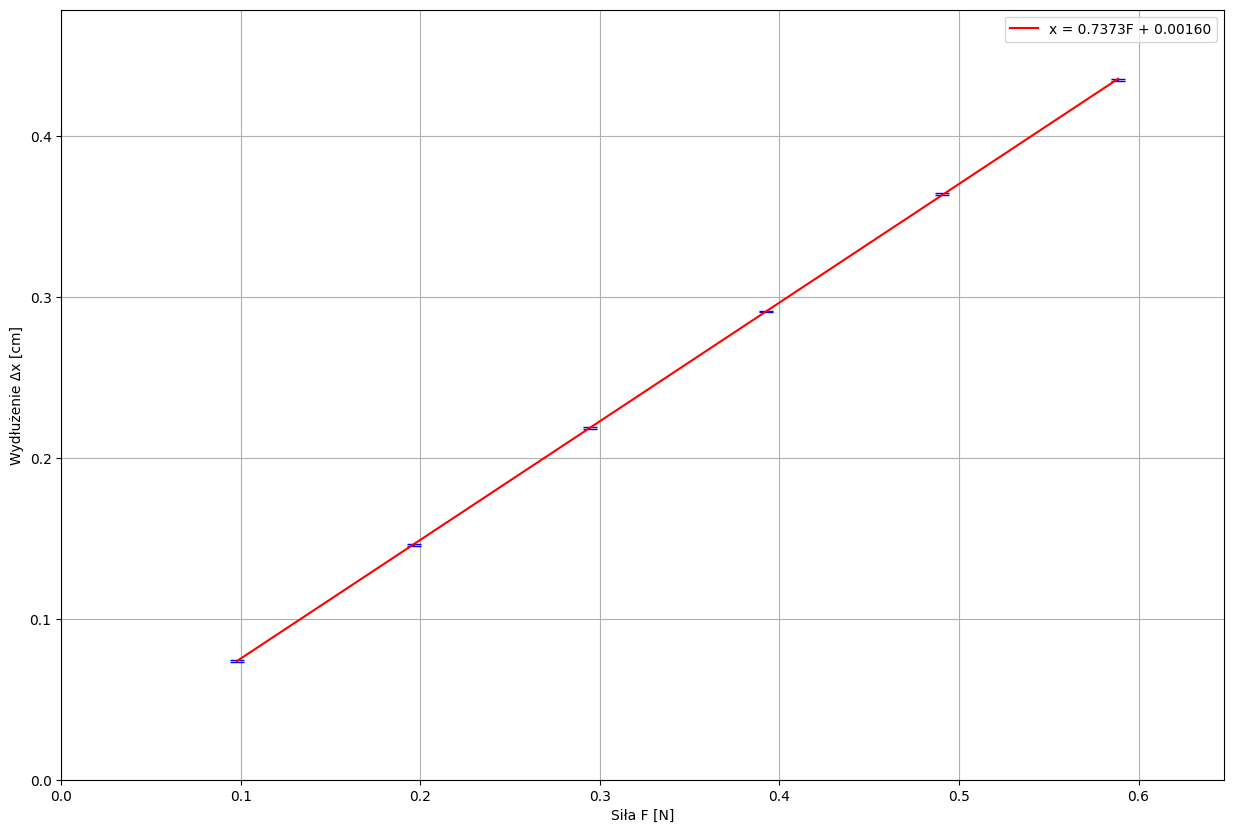
\includegraphics[width=1.2\linewidth,angle=90]{2-x(F).png}
    \caption{Zależność wydłużenia sprężyny od ciężaru (źródło: opracowanie własne).}
    \label{fig:zaleznosci}
\end{figure}


\bibliographystyle{plain}
\bibliography{bibliography}

\end{document}
